% Speed-strength plane for Marburg outbreaks (pooled generation interval).
% x = intrinsic growth rate r (day^-1), 95% CI as a horizontal whisker.
% y = mean generation interval T_g (days). Each outbreak sits at the mean of
%     its own transmission pairs where available (Tanzania 2023, n=7 -> 10.0 d)
%     otherwise the pooled Marburg serial interval 9.2 d (Qian et al. 2023,
%     medRxiv 10.1101/2022.06.17.22276538); the short vertical whisker is the
%     uncertainty in that mean. The shaded band is the pooled GI distribution
%     spread 9.2 +/- 4.4 d.
% R0 contours use the gamma GI form R0 = (1 + r*T_g/kappa)^kappa at the pooled
%     CV = 4.4/9.2 = 0.478 (kappa = 1/CV^2 = 4.38), so T_g = kappa*(R0^{1/kappa}-1)/r.
%     Point R0 estimates are in outbreak_R0_montecarlo.csv.
%
% Compile with pdflatex (or lualatex) + pgfplots (>= 1.16).
\documentclass[border=3pt]{standalone}
\usepackage{pgfplots}
\pgfplotsset{compat=1.16}
\usepackage{amsmath}

\definecolor{oiOrange}{RGB}{230,159,0}
\definecolor{oiGreen}{RGB}{0,158,115}
\definecolor{oiBlue}{RGB}{0,114,178}
\definecolor{oiVermil}{RGB}{213,94,0}
\definecolor{oiBlack}{RGB}{0,0,0}

\begin{document}
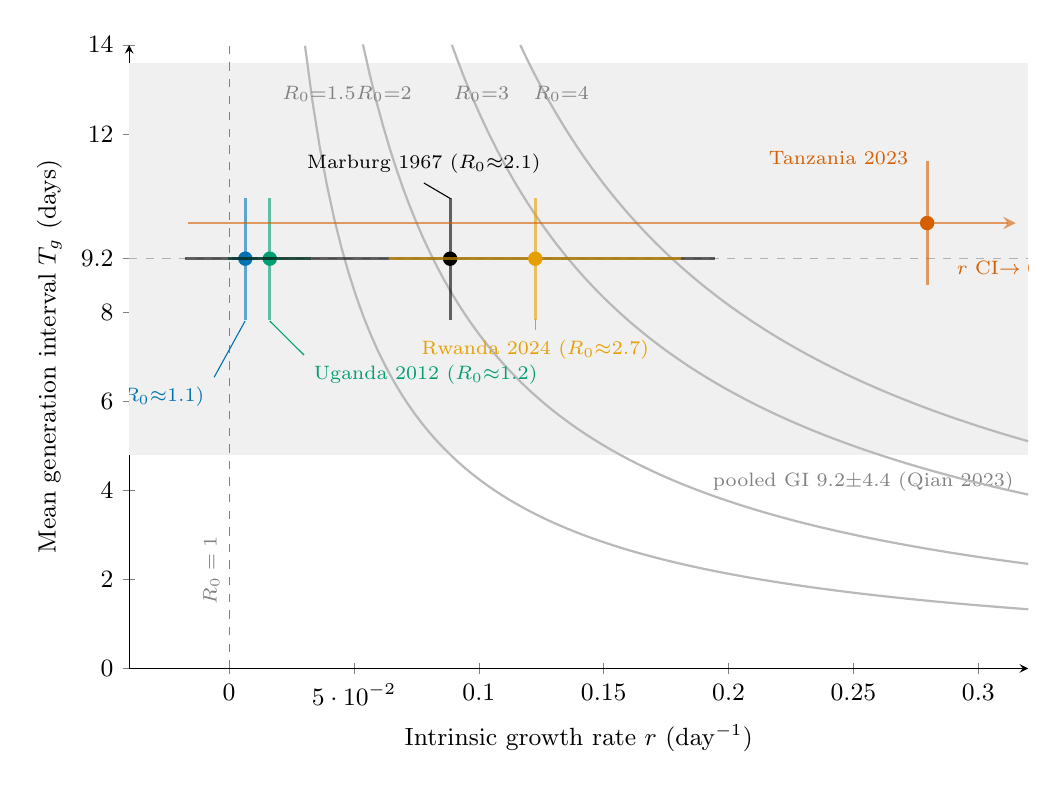
\begin{tikzpicture}
\begin{axis}[
    width=13cm, height=9.5cm,
    xlabel={Intrinsic growth rate $r$ (day$^{-1}$)},
    ylabel={Mean generation interval $T_g$ (days)},
    xmin=-0.04, xmax=0.32, ymin=0, ymax=14,
    axis lines=left,
    xtick={0,0.05,0.10,0.15,0.20,0.25,0.30},
    ytick={0,2,4,6,8,9.2,12,14}, yticklabels={0,2,4,6,8,9.2,12,14},
    tick label style={font=\small}, label style={font=\small}, clip=true,
]

% ---- pooled GI distribution spread 9.2 +/- 4.4 ----
\fill[gray!12] (axis cs:-0.04,4.8) rectangle (axis cs:0.32,13.6);
\draw[gray!60,dashed] (axis cs:-0.04,9.2) -- (axis cs:0.32,9.2);
\node[gray,font=\scriptsize,anchor=east] at (axis cs:0.318,4.2){pooled GI 9.2$\pm$4.4 (Qian 2023)};

% ---- gamma-GI R0 contours at CV=0.478: T_g = c/r ----
\addplot[gray!55,thick,domain=0.0304:0.32,samples=100]{0.425/x};
\addplot[gray!55,thick,domain=0.0536:0.32,samples=100]{0.751/x};
\addplot[gray!55,thick,domain=0.0892:0.32,samples=100]{1.249/x};
\addplot[gray!55,thick,domain=0.1166:0.32,samples=100]{1.632/x};
\node[gray,font=\scriptsize] at (axis cs:0.036,12.9){$R_0{=}1.5$};
\node[gray,font=\scriptsize] at (axis cs:0.062,12.9){$R_0{=}2$};
\node[gray,font=\scriptsize] at (axis cs:0.101,12.9){$R_0{=}3$};
\node[gray,font=\scriptsize] at (axis cs:0.133,12.9){$R_0{=}4$};

% ---- R0 = 1 threshold ----
\draw[gray,dashed] (axis cs:0,0) -- (axis cs:0,14);
\node[gray,font=\scriptsize,rotate=90,anchor=south] at (axis cs:0,2.2){$R_0=1$};

% \pt{r}{rlo}{rhi}{tg}{tglo}{tghi}{color}  (horizontal r CI + vertical mean-SE)
\newcommand{\pt}[7]{%
  \draw[#7,opacity=0.6,line width=1pt] (axis cs:#2,#4) -- (axis cs:#3,#4);%
  \draw[#7,opacity=0.6,line width=1pt] (axis cs:#1,#5) -- (axis cs:#1,#6);%
  \fill[#7] (axis cs:#1,#4) circle (2.6pt);%
}
% pooled T_g = 9.2, mean-SE band 7.83-10.57; r is the negative binomial estimate
\pt{0.0065}{0.0012}{0.0117}{9.2}{7.83}{10.57}{oiBlue}     % DRC 1999
\pt{0.0163}{-0.0003}{0.0329}{9.2}{7.83}{10.57}{oiGreen}   % Uganda 2012 (NB=Poisson)
\pt{0.0885}{-0.0175}{0.1945}{9.2}{7.83}{10.57}{oiBlack}   % Marburg 1967
\pt{0.1226}{0.0642}{0.1811}{9.2}{7.83}{10.57}{oiOrange}   % Rwanda 2024
% Tanzania 2023: own pair mean 10.0 (SE band 8.6-11.4); upper r CI 0.575 off-axis
\draw[oiVermil,opacity=0.6,line width=1pt,-stealth] (axis cs:-0.0164,10.0) -- (axis cs:0.315,10.0);
\draw[oiVermil,opacity=0.6,line width=1pt] (axis cs:0.2795,8.6) -- (axis cs:0.2795,11.4);
\fill[oiVermil] (axis cs:0.2795,10.0) circle (2.6pt);

% ---- labels with leader lines ----
\node[oiBlue,font=\scriptsize,anchor=east] (d) at (axis cs:-0.006,6.1){DRC 1999 ($R_0{\approx}1.1$)};
\draw[oiBlue,thin] (d.north east) -- (axis cs:0.0064,7.8);
\node[oiGreen,font=\scriptsize,anchor=west] (u) at (axis cs:0.03,6.6){Uganda 2012 ($R_0{\approx}1.2$)};
\draw[oiGreen,thin] (u.north west) -- (axis cs:0.0163,7.8);
\node[oiBlack,font=\scriptsize,anchor=south] (m) at (axis cs:0.078,10.9){Marburg 1967 ($R_0{\approx}2.1$)};
\draw[oiBlack,thin] (m.south) -- (axis cs:0.0886,10.55);
\node[oiOrange,font=\scriptsize,anchor=north] (rw) at (axis cs:0.1226,7.6){Rwanda 2024 ($R_0{\approx}2.7$)};
\draw[oiOrange,thin] (rw.north) -- (axis cs:0.1226,7.85);
\node[oiVermil,font=\scriptsize,anchor=south] at (axis cs:0.244,11.1){Tanzania 2023};
\node[oiVermil,font=\scriptsize,anchor=west] at (axis cs:0.286,9.0){\,$r$ CI$\to0.58$};

\end{axis}
\end{tikzpicture}
\end{document}
